\section{Mapper theory}
\label{sec:mapper}

This section defines Mapper, explains when it recovers the shape of the
data (the nerve lemma), relates it to the Reeb graph, and states the
known stability and parameter-selection results. A worked example on a
circle closes the section.

\paragraph{Notation.}
Throughout, $X$ is a topological space (in practice a point cloud
$X_n = \{x_1,\dots,x_n\} \subset \mathbb{R}^D$), $f\colon X \to \mathbb{R}$ a
continuous \emph{lens} (or filter), $\mathcal{I} = \{I_1,\dots,I_m\}$ a cover
of $f(X)$ by open intervals, $\mathcal{V}$ the refined pullback cover,
$N(\cdot)$ the nerve, $M_f(X,\mathcal{I})$ the Mapper graph,
$\bar M_f(X,\mathcal{I})$ the MultiNerve Mapper, $R_f(X)$ the Reeb
graph and $\tilde f$ the map it inherits from $f$. $\mathrm{Dg}(\cdot)$ is an
extended persistence diagram and $d_B$ the bottleneck distance. The
resolution $r$ is the length of the intervals, the gain $g$ the fraction
of an interval shared with the next one, and $\delta$ the scale of the
neighbourhood graph used for clustering.

\subsection{Construction}

\begin{definition}[Pullback cover]
Let $\mathcal{I}$ be a cover of $f(X)$. The \emph{pullback cover} of $X$ is
$f^{-1}(\mathcal{I}) = \{f^{-1}(I) : I \in \mathcal{I}\}$. Its
\emph{refinement} $\mathcal{V}$ splits each $f^{-1}(I)$ into its
path-connected components $V_{I,1},\dots,V_{I,c(I)}$; $\mathcal{V}$ is
again a cover of $X$, called the connected pullback
cover~\cite{carriere2018structure}.
\end{definition}

On a finite point cloud there are no connected components, so the
refinement step is replaced by a \emph{clustering} of each preimage
$f^{-1}(I) \cap X_n$. A common choice, used in the theory below, is to take
the connected components of the $\delta$-neighbourhood graph (an edge joins
two points at distance at most $\delta$), which is single-linkage
clustering cut at height~$\delta$~\cite{carriere2018statistical}.

\begin{definition}[Nerve]
The \emph{nerve} $N(\mathcal{V})$ of a cover $\mathcal{V} = \{V_\alpha\}$ is the
simplicial complex with one vertex per element and one $k$-simplex for every
$k+1$ elements with non-empty common intersection.
\end{definition}

\begin{definition}[Mapper~\cite{singh2007topological, carriere2018structure}]
The \emph{Mapper} of $(X,f)$ with cover $\mathcal{I}$ is
$M_f(X,\mathcal{I}) = N(\mathcal{V})$. The \emph{Mapper graph} is its
1-skeleton: one node per cluster, and an edge between two clusters that
share at least one point.
\end{definition}

If consecutive intervals overlap but no three intervals meet, as in the
usual cover with gain $g < 1/2$, no three elements of $\mathcal{V}$ meet
either, so $N(\mathcal{V})$ is already a graph~\cite[Lemma
2.12]{carriere2018structure}. The Mapper graph is then the whole Mapper.

\subsection{The nerve lemma and why Mapper covers break it}

A cover is \emph{good} if every non-empty finite intersection of its
elements is contractible.

\begin{theorem}[Nerve lemma~{\cite[Cor.~4G.3]{hatcher2002algebraic}}]
\label{thm:nerve}
If $\mathcal{U}$ is an open cover of a paracompact space $X$ such that every
non-empty intersection of finitely many sets in $\mathcal{U}$ is
contractible, then $X$ is homotopy equivalent to $N(\mathcal{U})$.
\end{theorem}

When it applies, the Mapper has the same loops and connected components as
$X$. Mapper covers, however, often fail the hypothesis, for two reasons.
First, an element $f^{-1}(I)$ may be connected but not contractible (it may
contain a loop), and clustering cannot fix this. Second, and more often,
the \emph{intersection} of two clusters may be disconnected. The nerve
records only whether an intersection is empty, so two separate overlaps
between the same pair of clusters become a single edge and the loop they
close is lost. The coarse cover in Figure~\ref{fig:toy-bad} shows this
case. Carri\`ere and Oudot fix it with the \emph{MultiNerve Mapper}, which
adds one edge per connected component of each
intersection~\cite[Sec.~3]{carriere2018structure}.

\subsection{The Reeb graph and Mapper as its approximation}

\begin{definition}[Reeb graph~{\cite[Def.~2.6]{carriere2018structure}}]
For $x,y\in X$ let $x \sim_f y$ if $f(x)=f(y)$ and $x,y$ lie in the same
connected component of $f^{-1}(f(x))$. The \emph{Reeb graph} is the
quotient $R_f(X) = X/{\sim_f}$, and $f$ induces a map
$\tilde f\colon R_f(X)\to\mathbb{R}$.
\end{definition}

The Reeb graph collapses each connected piece of each level set to a
point. It is a graph when $f$ is of \emph{Morse type}: $f$ has finitely
many critical values, between consecutive critical values $X$ is a product
$Y_i \times (a_i,a_{i+1})$ on which $f$ is the projection to the second
factor (with $Y_i$ compact and locally connected), these product
structures extend continuously to the closed intervals, and every level
set has finitely generated homology~\cite[Def.~2.1]{carriere2018structure}.
Mapper replaces level sets $f^{-1}(t)$ by preimages of intervals
$f^{-1}(I)$, so it is a \emph{pixelised} Reeb graph whose resolution is the
length of the intervals.

The features of a Reeb graph (connected components, loops and branches
pointing up or down) are summarised by the extended persistence diagram
$\mathrm{Dg}(\tilde f)$: one point $(x,y)$ per feature, whose coordinates are
the values of $f$ where the feature starts and ends, so that $|y-x|$ is its
size~\cite[Sec.~2]{carriere2018structure}. Carri\`ere and Oudot define the
diagram $\mathrm{Dg}(M_f(X,\mathcal{I}))$ of the Mapper as $\mathrm{Dg}(\tilde f)$
minus the points that fall into \emph{staircases}, regions of the plane
determined by the intervals of $\mathcal{I}$. A feature is lost exactly when
it fits inside one interval or one overlap. The result below uses
\emph{gomics}: covers by open intervals that are minimal (no element can
be removed) and generic (in the sense of~\cite[Sec.~2.5]{carriere2018structure}).
The \emph{granularity} of $\mathcal{I}$ is the length of its longest
interval.

\begin{theorem}[{\cite[Thm.~4.3 and Cor.~4.6]{carriere2018structure}}]
\label{thm:convergence}
Let $X$ be a topological space, $f\colon X\to\mathbb{R}$ a Morse-type function
and $\mathcal{I}$ a gomic of $f(X)$ with granularity at most $\varepsilon$. Let
$\bar M_f(X,\mathcal{I})$ be the MultiNerve Mapper. Then
\[
  \mathrm{Dg}(\tilde f) \setminus \{(x,y) : |y-x| \le \varepsilon\}
  \;\subseteq\; \mathrm{Dg}(\bar M_f(X,\mathcal{I}))
  \;\subseteq\; \mathrm{Dg}(\tilde f),
\]
and hence $d_B\bigl(\mathrm{Dg}(\bar M_f(X,\mathcal{I})), \mathrm{Dg}(\tilde f)\bigr) \le \varepsilon/2$.
\end{theorem}

In words: every feature of the Reeb graph larger than the intervals
appears in the MultiNerve Mapper, which has no feature the Reeb graph
lacks, and as $\varepsilon \to 0$ it converges to the Reeb graph. The
ordinary Mapper is obtained by merging edges with the same endpoints.
This can only remove loops, namely those that fit inside the union
$I\cup J$ of two consecutive intervals~\cite[Sec.~4.3, Eq.~(6)]{carriere2018structure}.
So in the Mapper a loop is guaranteed to survive when it is larger than
every such union.

\subsection{Stability and parameter selection}

\paragraph{Stability under changes of the lens.}
Carri\`ere and Oudot define a distance $d_{\mathcal{I}}$ between Mapper
diagrams. It is the bottleneck distance, except that an unmatched point
pays its $\ell_\infty$ distance to the staircase of its type instead of to
the diagonal~\cite[Def.~5.1]{carriere2018structure}. This measures how far
a feature is from disappearing for the given cover.

\begin{theorem}[{\cite[Thm.~5.2]{carriere2018structure}}]
Let $X$ be a topological space, $f,f'\colon X\to\mathbb{R}$ Morse-type functions and
$\mathcal{I}$ a gomic. Then
\[
  d_{\mathcal{I}}\bigl(\mathrm{Dg}(M_f(X,\mathcal{I})),\,\mathrm{Dg}(M_{f'}(X,\mathcal{I}))\bigr)
  \le \|f-f'\|_\infty .
\]
\end{theorem}

The theorem is stated for the MultiNerve Mapper and holds for the Mapper
with the extended staircase of~\cite[Sec.~4.3]{carriere2018structure}. A
small change of the lens moves each feature by at most as much, measured
with respect to the cover. A feature close to its staircase, however, can
appear or disappear under a small perturbation, so it should not be
trusted.

\paragraph{Approximation from a sample.}
Carri\`ere, Michel and Oudot study the Mapper $M_n = M_{r,g,\delta}(X_n)$ built
on a sample $X_n$ of a space $X$. Its intervals have length $r$ (except the
first and last), consecutive intervals overlap by a fraction
$g \in (0,\tfrac12)$, and its clusters are the connected components of the
$\delta$-neighbourhood graph. Its distance to the Reeb graph, $d_\Delta$, is
the bottleneck distance between their extended persistence
diagrams~\cite[Sec.~2]{carriere2018statistical}. A \emph{modulus of
continuity} for $f$ is a function $\omega$ with
$|f(x)-f(x')|\le\omega(\|x-x'\|)$ that is non-negative, non-decreasing,
subadditive, continuous and has $\omega(0)=0$.

\begin{theorem}[{\cite[Thm.~2.7]{carriere2018statistical}}]
\label{thm:cmo}
Let $X$ be a smooth compact submanifold of $\mathbb{R}^D$ with positive reach
$\mathrm{rch}$ and convexity radius $\rho$, let $X_n \subset X$ be $n$ points,
and let $f$ be Morse-type on $X$ with modulus of continuity $\omega$. If
\begin{enumerate}
  \item[(1)] $\delta \le \tfrac14 \min\{\mathrm{rch},\rho\}$,
  \item[(2)] $\max\{|f(x)-f(x')| : x,x'\in X_n,\ \|x-x'\|\le\delta\} < g\,r$, and
  \item[(3)] $4\,d_H(X,X_n) \le \delta$, with $d_H$ the Hausdorff distance,
\end{enumerate}
then $d_\Delta\bigl(R_f(X), M_{r,g,\delta}(X_n)\bigr) \le r + 2\,\omega(\delta)$.
\end{theorem}

The hypotheses say that $\delta$ must be large enough to connect the sample
(3) but small enough not to short-cut the space (1), and that the
overlaps must be wider than the change of $f$ across one edge of the
neighbourhood graph (2), so that the clusters on both sides of an overlap
share points.

\paragraph{Parameter selection.}
From this theorem the same authors derive a rule that needs no
knowledge of $X$~\cite[Sec.~3.3]{carriere2018statistical}. Fix
$g\in(\tfrac13,\tfrac12)$. Take a random subsample $\hat X$ of
$s_n = n/(\log n)^{1+\beta}$ points, for some $\beta>0$, and set
\[
  \delta_n = d_H(\hat X, X_n), \qquad
  r_n = \frac{V_n(\delta_n)^+}{g},
\]
with $V_n(\delta) = \max\{|f(x)-f(x')| : x,x'\in X_n,\ \|x-x'\|\le\delta\}$,
where $V^+$ is a value slightly larger than $V$. Assume the points are
drawn i.i.d.\ from a distribution $P$ whose support is a smooth compact
submanifold (positive reach and convexity radius, bounded diameter) and
which is $(a,b)$-standard, i.e.\ $P(B(x,t))\ge\min(1,a t^b)$ for every ball,
and assume $\omega(x)/x$ is non-increasing. Then the expected value of
$d_\Delta(R_f(X), M_n)$ is at most
$C\,\omega\bigl((C'\log(n)^{2+\beta}/n)^{1/b}\bigr)$, which is minimax optimal
up to the logarithmic factor~\cite[Props.~3.3 and 3.4]{carriere2018statistical}.
Our embeddings are not known to satisfy these assumptions. We use the rule
as a principled default, not as a guarantee.

\subsection{Why a graph and not a clustering}

A flat clustering partitions the data and says nothing about how the
clusters relate. Mapper keeps two kinds of information that a partition
loses. First, \emph{neighbourhood}: an edge means two clusters share
points, so the regions they describe touch. The graph shows which topics
lie next to which, and paths, loops and branches show how they connect.
Second, \emph{structural change}: when data are added, a partition only
changes cluster sizes or labels, while the graph can show a new edge (two
regions now touch), a node that splits or merges, or a loop that appears
or closes. Each change points to a specific region of the data. This is
what our selector uses to decide which questions to re-test after an
ingestion.

\subsection{Worked example: a noisy circle}

We sample 300 points from the unit circle with Gaussian noise
($\sigma = 0.06$) and use the height $f(x,y)=y$ as lens. Its range is
covered by 6 intervals with gain $g = 0.3$, and each preimage is clustered
by single linkage at distance $0.25$ (Figure~\ref{fig:toy}). Bands crossing
the circle contain two arcs and give two clusters. The bands at the top and
bottom give one. The 10 clusters, joined where they share points, form a
graph with exactly one loop, the hole of the circle. Here the refined
cover is good: its elements are arcs and their pairwise intersections are
arcs, so Theorem~\ref{thm:nerve} applies to the underlying circle and the
nerve is a circle too.

\begin{figure}[ht]
  \centering
  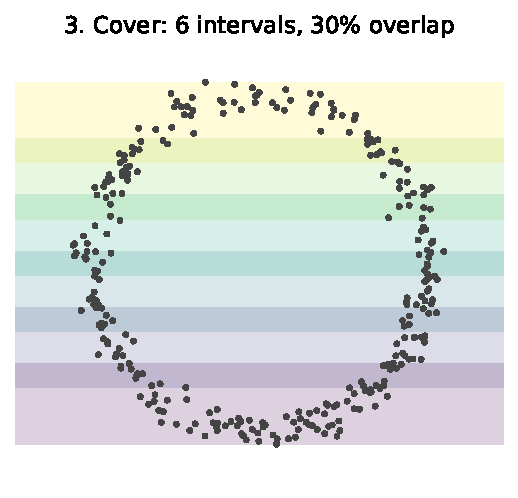
\includegraphics[width=0.31\textwidth]{figures/toy/03_cover.pdf}\hfill
  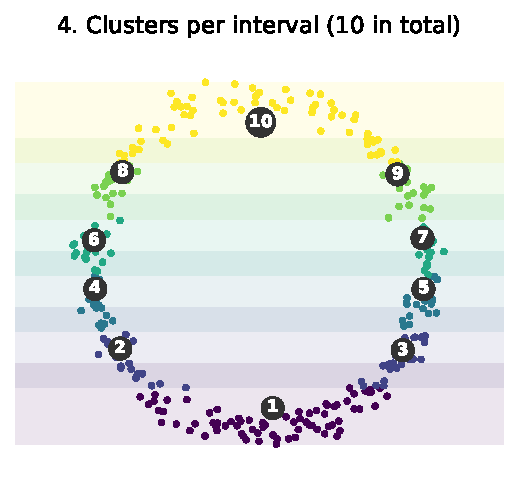
\includegraphics[width=0.31\textwidth]{figures/toy/04_clusters.pdf}\hfill
  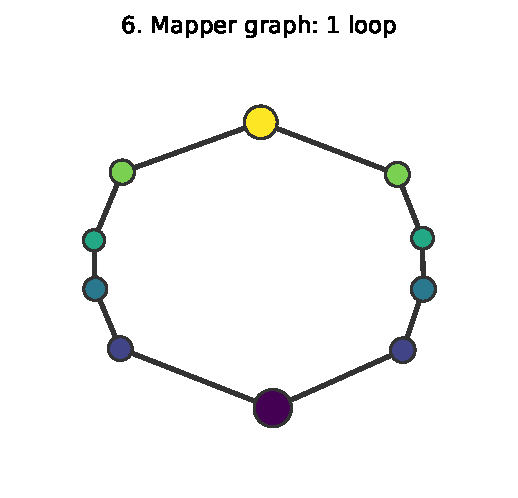
\includegraphics[width=0.31\textwidth]{figures/toy/06_graph.pdf}
  \caption{Mapper on a noisy circle. Left: the height range is covered by
  6 overlapping intervals. Centre: each band is clustered separately,
  giving 10 clusters. Right: the Mapper graph has one loop, the hole of
  the circle.}
  \label{fig:toy}
\end{figure}

Figure~\ref{fig:toy-bad} shows two covers that lose the loop. With only
two intervals (left), each band holds one arc. Their overlap has two
pieces, one on each side of the circle, so the intersection of the two
clusters is not connected and the cover is not good. The nerve records a
single edge and the graph is a segment. The MultiNerve Mapper would keep
both edges and the loop. With no overlap (right), no two clusters share a
point, the nerve has no edges and the graph falls apart into 10 isolated
nodes. Both failures match the theory. The Reeb graph of the height on the
circle is the circle itself, with one loop spanning the whole range
$[-1,1]$. With two intervals, their union is the whole range, so the loop
fits inside it and the Mapper may lose it, while each interval is shorter
than the loop, so the MultiNerve Mapper keeps it
(Theorem~\ref{thm:convergence}). Without overlap, the intervals no longer
form an open cover in which consecutive elements meet, so no result
applies and the graph is disconnected.

\begin{figure}[ht]
  \centering
  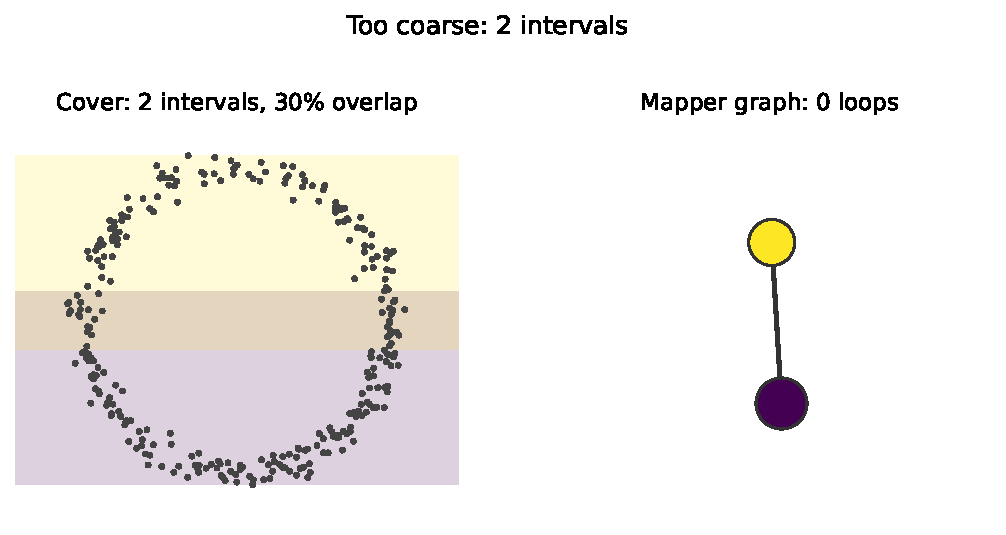
\includegraphics[width=0.48\textwidth]{figures/toy/07_bad_coarse.pdf}\hfill
  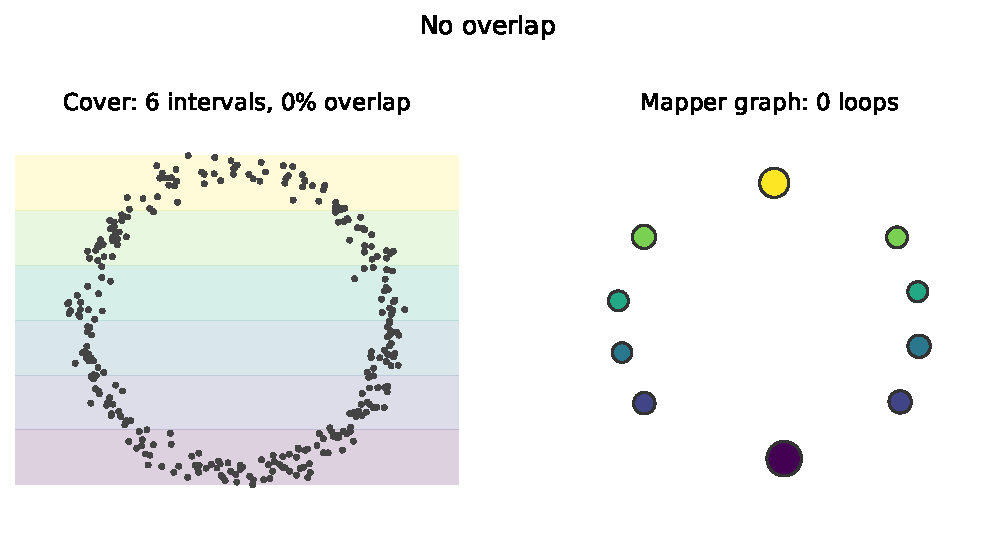
\includegraphics[width=0.48\textwidth]{figures/toy/08_bad_no_overlap.pdf}
  \caption{Bad covers. Left: two intervals; the overlap has two pieces but
  the nerve records one edge, so the loop is lost. Right: no overlap; the
  graph has no edges.}
  \label{fig:toy-bad}
\end{figure}
